\section{Resultados} \label{resultados}

A mesma base de teste (sendo 10 de cada classe, totalizando 30) foi usada para verificar tanto o desempenho das 3 redes que compõe a auto associativa, quanto da rede MLP.

O parâmetro de comparação foi o erro médio quadrático (MSE) obtido no desempenho das redes.


\subsection{Desempenho da Rede MLP}

A rede MLP apresentou um desempenho bom, tendo em vista que houve apenas 1 erro na classificação.

\begin{figure}[H]

\centering % para centralizarmos a figura
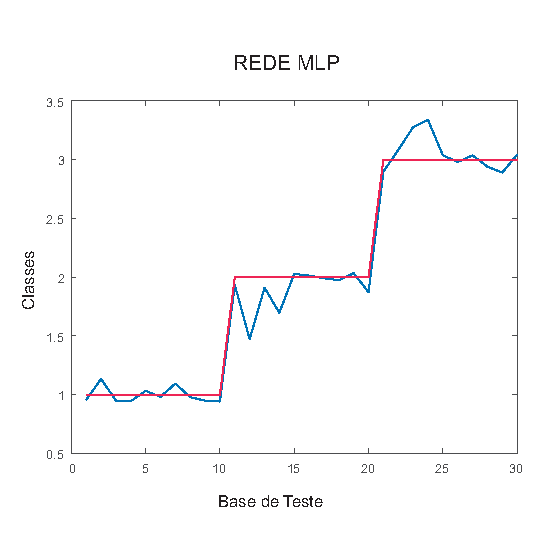
\includegraphics{04-Figuras/SAIDA_MLP}

\caption{Saída da rede MLP}

\label{figura:saidaMLP}

\end{figure}

A fig. \ref{figura:saidaMLP} mostra o desempenho da rede MLP, onde em azul é a saída da rede e em vermelho, a saída desejada.


\subsection{Desempenho da Rede Auto Associativa}

Considerando toda a base de teste (30 instâncias), as três redes que compõe a estrutura competitiva auto associativa apresentaram resultados bem interessantes para as classes nas quais elas são especializadas. No entanto, elas apresentaram erros consideráveis para as instâncias da base de teste pertencente às outras classes (o que de certa forma é esperado).





\begin{table}[H]
\centering
\caption{Desempenho de classificação da rede auto associativa}
\resizebox{\columnwidth}{!}{%
\begin{tabular}{cllcc}
\hline
TREINO & \multicolumn{3}{c}{MSE}                                                & CLASSIFICAÇÃO \\
                  & \multicolumn{1}{c}{REDE 1} & \multicolumn{1}{c}{REDE 2} & REDE 3       &               \\ \hline
1 a 10            & 8.5993e-06                 & 0.000851717                & 0.0246367908 & 1 (100\%)     \\
11 a 20           & 2.7620175                  & 8.67907e-19                & 1.5048243951 & 2 (100\%)     \\
21 a 30           & 0.253580                   & 0.26402623                 & 0.0003252681 & 3 (100\%)     \\ \hline
\end{tabular}%
}

\label{tabela:classificacao}

\end{table}



A Tabela \ref{tabela:classificacao} apresenta o desempenho geral da rede auto associativa. Quando a base de teste das três classes (30 instâncias) foram alimentadas na rede, houve 100\% de acertos na classificação dos dados, onde cada rede especializada obteve os menores erros médios quadráticos (MSE) possíveis para as instâncias as quais lhe pertenciam de fato. Nas Considerações Finais (Seção \ref{consideracoesFinais}) desde documento, fazemos uma discussão sobre a provável explicação para a rede auto associativa acertar em 100\%.

\subsubsection{Desempenho da Rede 1}

A fig. \ref{figura:rede1} mostra o desempenho da rede 1, que é especializada na classe 1.

\begin{figure}[H]

\centering % para centralizarmos a figura
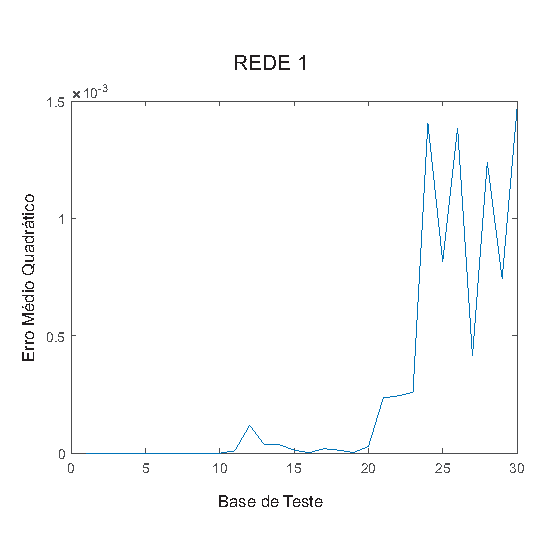
\includegraphics{04-Figuras/MSE_DesempenhoNet1}

\caption{Desempenho da rede 1}

\label{figura:rede1}

\end{figure}

Observa-se que o erro médio quadrático é extremamente baixo para a base de dados de 1 a 10 (que corresponde à classe 1) e bastante significativo entre 11 a 30, que são instâncias pertencentes às classes 2 e 3.

\subsubsection{Desempenho da Rede 2}

Na rede 2, o padrão de comportamento da rede 1 se repetiu. Observa-se que de 1 a 10 o MSE é acentuado, sendo extremamente baixo de 11 a 20 (instâncias pertencentes à classe 2), e novamente alto de 21 a 30, como mostrado na fig. \ref{figura:rede2}.

\begin{figure}[H]

\centering % para centralizarmos a figura
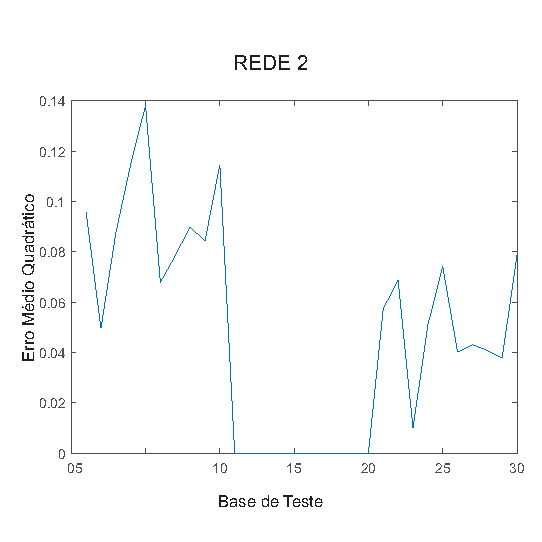
\includegraphics{04-Figuras/MSE_DesempenhoNet2}

\caption{Desempenho da rede 2}

\label{figura:rede2}

\end{figure}

\subsubsection{Desempenho da Rede 3}

Seguindo a tendência de comportamento, a rede 3 apresentou um alto valor do MSE para as instâncias de 1 a 20 (pertencentes às classes 1 e 2), bem como um erro muito baixo para as instâncias da classe 3, onde a rede 3 é especializada, de 21 a 30.

\begin{figure}[H]

\centering % para centralizarmos a figura
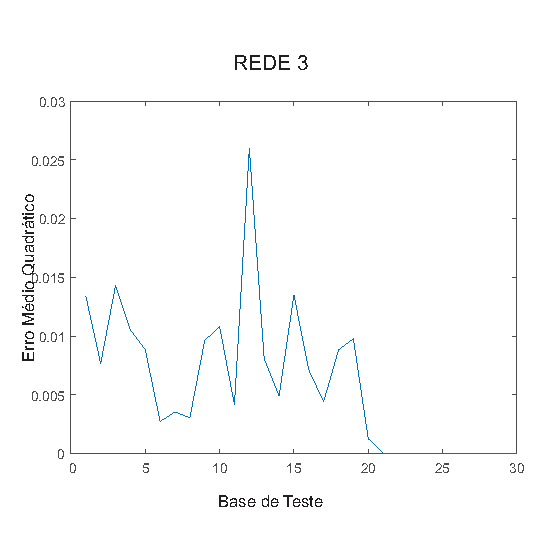
\includegraphics{04-Figuras/MSE_DesempenhoNet3}

\caption{Desempenho da rede 3}

\label{figura:rede3}

\end{figure}



\subsection{Comparação Rede MLP X Rede Auto Associativa}

Tabela de comparação entre as redes.


